\chapter{Fungsi dan Kelas}
Tujuan pembelajaran pada pertemuan ketiga antara lain:
\begin{enumerate}
\item
Mengenal struktur fungsi di python dalam satu file dan cara pemanggilannya
\item
Mengerti cara membuat library fungsi dan melakukan import dan berbagai jenis import
\item
Mengerti struktur library kelas python dan cara pemakaiannya
\item
Mengatasi Error yang terjadi akibat pemakaian fungsi dan kelas
\item
Try Except
\end{enumerate}
Tugas dengan cara dikumpulkan dengan pull request ke github dengan menggunakan latex pada repo yang dibuat oleh asisten IRC. Kode program dipisah dalam folder src NPM.py yang berisi praktek dari masing-masing tugas file terpisah sesuai nomor yang kemudian dipanggil menggunakan input listing ke dalam file latex penjelasan atau nomor pengerjaan. Masing masing soal bernilai 5 dengan total nilai 100. Gunakan bahasa yang baku dan bebas plagiat dengan dibuktikan hasil scan plagiarisme. Serta hasil scrinsut dari komputer sendiri, dan kode hasil sendiri.

\section{Contoh Program}
\subsection{Fungsi}
Fungsi adalah satu blok program yang terdiri dari nama fungsi, input variabel dan variabel kembalian. Nama fungsi diawali dengan \textit{def} dan setelahnya tanda titik dua. Nama bisa sama dengan isi berbeda jika menggunakan huruf besar dan kecil atau sering disebut dengan \textit{case sensitive}. Input variabel bisa lebih dari satu dengan pemisah tanda koma. variabel kembalian pasti satu, bebas apakan itu jenis \textit{string}, \textit{integer}, \textit{list} atau \textit{dictionary}. Contoh dari fungsi sederhana bisa dilihat pada listing \ref{lst:fungsisederhana}. Dimana hasil akhir variabel c adalah 15.
\begin{lstlisting}[caption=Fungsi Sederhana,label={lst:fungsisederhana}]
def Penambahan(a,b):
	r = a + b
	return r
	
	
a=2
b=13
c = Penambahan(a,b)
\end{lstlisting}
sekarang kita pisah fungsi dengan pemakaian fungsi tersebut dalam file terpisah. Kita buat file bernama \textit{kalkulator.py} yang berisi semua fungsi penambahan, pengurangan, perkalian dan pembagian seperti terlihat pada listing \ref{lst:kalkulatorlib}. Sehingga satu file yang hanya berisi semua fungsi ini kita namakan \textit{paket} atau \textit{library}.
\begin{lstlisting}[caption=Library atau Paket kalkulator,label={lst:kalkulatorlib}]
def Penambahan(a,b):
	r = a + b
	return r
def Pengurangan(a,b):
	r = a - b
	return r
def Perkalian(a,b):
	r = a * b
	return r
def Pembagian(a,b):
	r = a / b
	return r
\end{lstlisting}
	Dan satu file yang memakai fungsi tersebut dengan nama file \textit{main.py}. Karena file kalkulator.py merupakan sebuah library maka kita panggil dulu dengan menggunakan perintah \textit{import}. Harus diingat file \textit{kalkulator.py} harus satu folder dengan \textit{main.py} yang berisi seperti listing\ref{lst:pakaikalkulator}.
\begin{lstlisting}[caption=Cara penggunaan library kalkulator,label={lst:pakaikalkulator}]
import kalkulator

a=100
b=50
hasil1=kalkulator.Penambahan(a,b)
hasil2=kalkulator.Pengurangan(a,b)
hasil3=kalkulator.Perkalian(a,b)
hasil4=kalkulator.Pembagian(a,b)
\end{lstlisting}
Maka kita bisa lihat hasilnya pada variabel hasil1, hasil2, hasil3, hasil4. Pada variabel exporer di spyder.

\subsection{Kelas}
Dasarnya dari kelas adalah pemrograman berbasis objek. Maka kita harus ingat, ada kelas ada objek ada atribut ada method. Fungsi kalkulator kita ubah menjadi kelas Ngitung.py menjadi seperti pada listing \ref{lst:kelasngitung}.
\begin{lstlisting}[caption=Kelas library kalkulator,label={lst:kelasngitung}]
class Ngitung:
  def __init__(self, a, b):
    self.a = a
    self.b = b
  def Penambahan(self):
    r = self.a + self.b
    return r
  def Pengurangan(self):
    r = self.a - self.b
    return r
  def Perkalian(self):
    r = self.a * self.b
    return r
  def Pembagian(self):
    r = self.a / self.b
    return r
\end{lstlisting}
Dana pada file main.py untuk menggunakan kelas maka bedanya adalah penambahan variabel yang menjadi objek instansiasi dari kelas seperti terlihat pada listing \ref{lst:instanngitung}.
\begin{lstlisting}[caption=Cara penggunaan kelas library kalkulator,label={lst:instanngitung}]
import ngitung

a=100
b=50

hitung = ngitung.Ngitung(a,b)

hasil1=hitung.Penambahan()
hasil2=hitung.Pengurangan()
hasil3=hitung.Perkalian()
hasil4=hitung.Pembagian()
\end{lstlisting}



\section{Pemahanan Teori}
Kerjakan soal berikut ini, masing masing bernilai 5. 
Praktek teori penunjang yang dikerjakan :
\begin{enumerate}
\item
Apa itu fungsi, inputan fingsi dan kembalian fungsi dengan contoh kode program lainnya.
\par\textbf{Jawaban} Fungsi adalah sebuah atau satu blok kode program yang dapat di eksekusi di bagian lain dalam suatu program.
\item
Apa itu paket dan cara pemanggilan paket atau library dengan contoh kode program lainnya.
\par\textbf{Jawaban} Paket adalah sebuah file yang berisi fungsi perkalian,pembagian,pengurangan dan penambahan, cara penmanggilannya yaitu dengan cara import
\item
Jelaskan Apa itu kelas, apa itu objek, apa itu atribut, apa itu method dan contoh kode program lainnya masing-masing.
\par\textbf{Jawaban} 
\begin{itemize}
    \item Kelas adalah klasifikasi dari objek
        \begin{center}
        \centering
        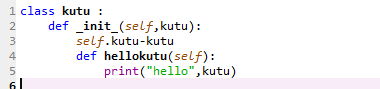
\includegraphics[scale=1]{figures/chapter 3/1.PNG}
    \end{center}
    \item objek adalah instansi dari kelas
    \begin{center}
        \centering
        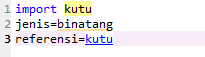
\includegraphics[scale=1]{figures/chapter 3/2.PNG}
    \end{center}
    \item atribut adalah presentasi dari suatu kelas 
        \begin{center}
        \centering
        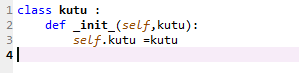
\includegraphics[scale=1]{figures/chapter 3/3.PNG}
    \end{center}
    \item method adalah fungsi pada suatu program itu sendiri
            \begin{center}
        \centering
        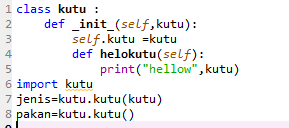
\includegraphics[scale=1]{figures/chapter 3/4.PNG}
    \end{center}
\end{itemize}
\item
Jelaskan cara pemanggikan library kelas dari instansiasi dan pemakaiannya dengan contoh program lainnya.
\par \textbf{Jawban}
        \begin{center}
        \centering
        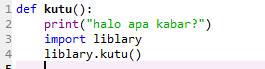
\includegraphics[scale=1]{figures/chapter 3/5.PNG}
    \end{center}
\item
Jelaskan dengan contoh pemakaian paket dengan perintah \textit{from kalkulator import Penambahan} disertai dengan contoh kode lainnya.
\par\textbf{Jawaban} dari class dengan cara menambahkan variabel yang menjadi instansi dari class itu sendiri
\item
Jelaskan dengan contoh kodenya, pemakaian paket fungsi apabila file library ada di dalam folder.
\par\textbf{Jawaban} dengan cara memanggil nama foldernya lalu nama liblarynya
        \begin{center}
        \centering
        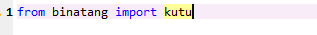
\includegraphics[scale=1]{figures/chapter 3/6.PNG}
    \end{center}
\item
Jelaskan dengan contoh kodenya, pemakaian paket kelas apabila file library ada di dalam folder.
\par\textbf{Jawaban} dengan cara memangil nama foldernya lalu nama classnya
        \begin{center}
        \centering
        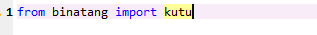
\includegraphics[scale=1]{figures/chapter 3/6.PNG}
    \end{center}
\end{enumerate}

\section{Ketrampilan Pemrograman}
Kerjakan soal berikut ini, masing masing bernilai 5. Pada pertemuan sebelumnya tentang pembuatan program di python, sekarang cobalah untuk membuat nya dalam bentuk fungsi dan kelas dengan ketentuan:
\begin{enumerate}
\item
Buatlah fungsi dengan inputan variabel NPM, dan melakukan print luaran huruf yang dirangkai dari tanda bintang, pagar atau plus dari NPM kita.
Tanda bintang untuk NPM mod 3=0, tanda pagar untuk NPM mod 3 =1, tanda plus untuk NPM mod3=2.
Contoh Output : 
\begin{verbatim}
*****    *** ******     *****    ****
*******  *** ***  **    *** **  *****
***  ******* ******     ***  **** ***
***    ***** ***        ***       ***
***     **** ***        ***       ***
\end{verbatim}
NPM sesuai dengan nomor NPM nya.
\par\textbf{Jawaban}
        \begin{center}
        \centering
        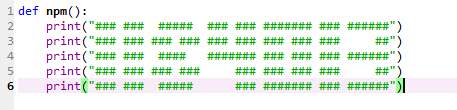
\includegraphics[scale=1]{figures/chapter 3/7.PNG}
    \end{center}
\item
Buatlah fungsi dengan inputan variabel berupa NPM. kemudian dengan menggunakan perulangan mengeluarkan print output sebanyak dua dijit belakang NPM, 
contoh NPM : 113040087 maka akan ada output sebanyak 87 dengan tulisan `Hallo, 113040087 apa kabar?'
\begin{verbatim}
Output : 
Halo, 113040087 apa kabar? 
Halo, 113040087 apa kabar?
Halo, 113040087 apa kabar?
Halo, 113040087 apa kabar?
Halo, 113040087 apa kabar?
Halo, 113040087 apa kabar?
Halo, 113040087 apa kabar?
Halo, 113040087 apa kabar?
.....87 kali...
\end{verbatim}
\par\textbf{Jawaban}
        \begin{center}
        \centering
        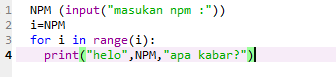
\includegraphics[scale=1]{figures/chapter 2/15.PNG}
    \end{center}
\item
Buatlah fungsi dengan dengan input variabel string bernama \textbf{NPM} dan beri luaran output dengan perulangan berupa tiga karakter belakang dari NPM sebanyak penjumlahan tiga dijit tersebut. Penjumlahan dilakukan dengan menggunakan operator aritmatika dan fungsi int() atau str().
\begin{verbatim}
Output : Halo, Nama apa kabar? 
Halo, 087 apa kabar?
Halo, 087 apa kabar?
Halo, 087 apa kabar?
Halo, 087 apa kabar?
Halo, 087 apa kabar?
Halo, 087 apa kabar?
Halo, 087 apa kabar?
........15 kali(0+8+7).........
\end{verbatim}
\par\textbf{Jawaban}
        \begin{center}
        \centering
        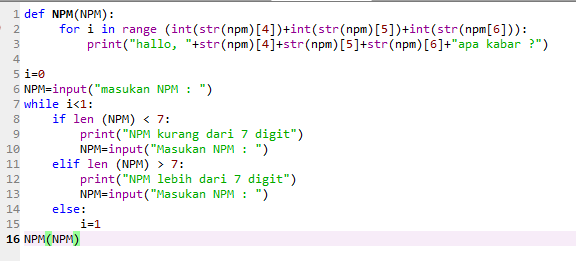
\includegraphics[scale=1]{figures/chapter 3/8.PNG}
    \end{center}
\item
Buatlah fungsi hello word dengan input variabel string bernama \textbf{NPM} dan beri luaran output berupa digit ketiga dari belakang dari variabel NPM menggunakan akses langsung manipulasi string pada baris ketiga dari variabel NPM.
\begin{verbatim}
Input : 113040087
Output :
Halo, 0 apa kabar?
\end{verbatim}
\par\textbf{Jawaban}
        \begin{center}
        \centering
        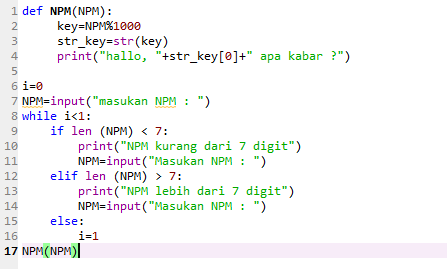
\includegraphics[scale=1]{figures/chapter 3/9.PNG}
    \end{center}
\item

\label{digitvar2}
(wajib menggunakan perulangan dan atau kondisi) buat fungsi program dengan input variabel NPM dan melakukan print nomor npm satu persatu kebawah.
Contoh untuk NPM : 113040087 maka,
\begin{verbatim}
1
1
3
0
4
0
0
8
7
\end{verbatim}
\par\textbf{Jawaban}
        \begin{center}
        \centering
        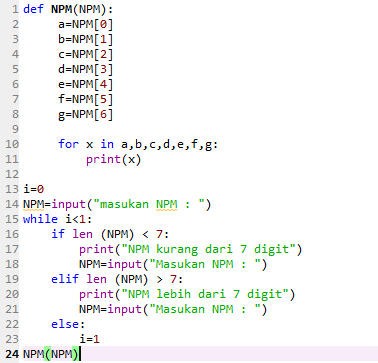
\includegraphics[scale=1]{figures/chapter 3/10.PNG}
    \end{center}
\item
Buatlah fungsi dengan inputan variabel NPM, didalamnya melakukan penjumlahan dari seluruh dijit NPM tersebut, wajib menggunakan perulangan dan atau kondisi.
\par\textbf{Jawaban}
      \begin{center}
        \centering
        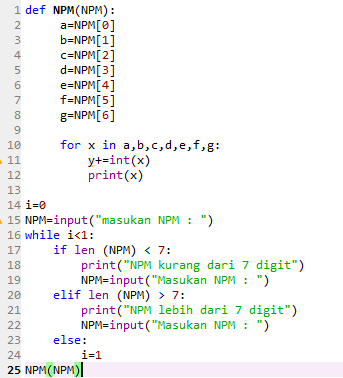
\includegraphics[scale=1]{figures/chapter 3/11.PNG}
    \end{center}
\item 
Buatlah fungsi dengan inputan variabel NPM, didalamnya melakukan melakukan perkalian dari seluruh dijit NPM tersebut, wajib menggunakan perulangan dan atau kondisi.
\par\textbf{Jawaban}
      \begin{center}
        \centering
        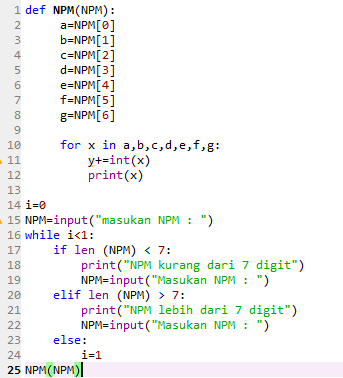
\includegraphics[scale=1]{figures/chapter 3/11.PNG}
    \end{center}

\item
Buatlah fungsi dengan inputan variabel NPM, Lakukan print NPM anda tapi hanya dijit genap saja. wajib menggunakan perulangan dan atau kondisi. Contoh jika NPM :113040087.
\begin{verbatim}
48
\end{verbatim}
\par\textbf{Jawaban}
      \begin{center}
        \centering
        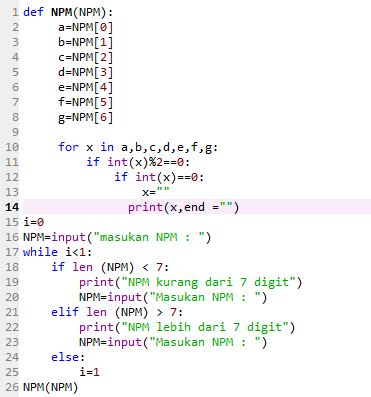
\includegraphics[scale=1]{figures/chapter 3/12.PNG}
    \end{center}
\item
Buatlah fungsi dengan inputan variabel NPM, Lakukan print NPM anda tapi hanya dijit ganjil saja. wajib menggunakan perulangan dan atau kondisi. Contoh jika NPM :113040087.
\begin{verbatim}
1137
\end{verbatim}
\par\textbf{Jawaban}
      \begin{center}
        \centering
        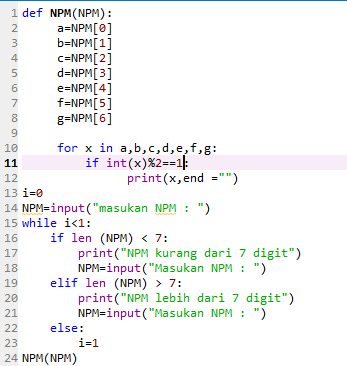
\includegraphics[scale=1]{figures/chapter 3/13.PNG}
    \end{center}
\item 
Buatlah fungsi dengan inputan variabel NPM, Lakukan print NPM anda tapi hanya dijit yang termasuk bilangan prima saja. wajib menggunakan perulangan dan atau kondisi. Contoh jika NPM :113040087.
\begin{verbatim}
37
\end{verbatim}
\item
Buatlah satu library yang berisi fungsi-fungsi dari nomor diatas dengan nama file 3lib.py dan berikan contoh cara pemanggilannya pada file main.py.
\item
Buatlah satu library class dengan nama file kelas3lib.py yang merupakan modifikasi dari fungsi-fungsi nomor diatas dan berikan contoh cara pemanggilannya  pada file main.py.
\end{enumerate}


\section{Ketrampilan Penanganan Error}
Kerjakan soal berikut ini, masing masing bernilai 5. Bagian Penanganan error dari script python.
\begin{enumerate}
\item
Tuliskan peringatan error yang didapat dari mengerjakan praktek ketiga ini, dan jelaskan cara penanganan error tersebut.
dan Buatlah satu fungsi yang menggunakan gunakan try except untuk menanggulangi error yang kemungkinan akan terjadi.
\par\textbf{Jawaban}
\begin{itemize}
    \item  berikut errornya yaitu penggunaan variable yang tidak tepat
      \begin{center}
        \centering
        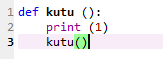
\includegraphics[scale=1]{figures/chapter 3/14.PNG}
    \end{center}
    
        \item  cara penanganannya
      \begin{center}
        \centering
        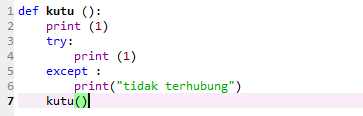
\includegraphics[scale=1]{figures/chapter 3/15.PNG}
    \end{center}
    
    \end{itemize}
\end{enumerate}

